

\begin{figure}[ht]
\begin{center}
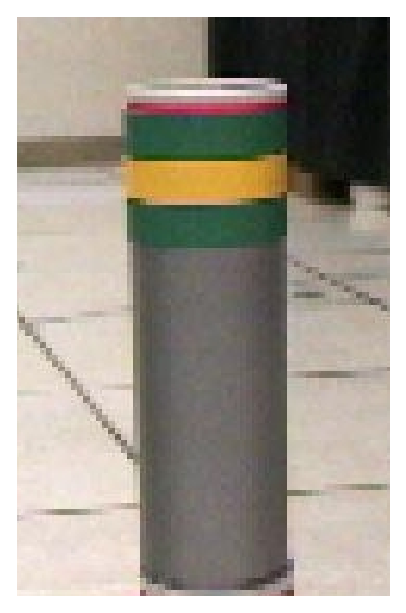
\epsfig{file=laservisualbeacon.eps, height=40mm}
\caption{A sample laser visual barcode.}
\label{fig:laservisualbarcode}
\end{center}
\end{figure}

\subsection*{Synopsis}

The laser visual barcode detector uses both searches for fiducials
that are both retro-reflective and color-coded.  Fiducials can be
either planar or cylindical, as shown in Figure
\ref{fig:laservisualbarcode}.  For planar targets, the range, bearing,
orientation and identity will be determined; for cylindrical targets,
the orientation will be undefined.  The target size and shape can be
set in the configuration file.

The laser visual barcode detector searches the laser range data to
find retro-reflective targets, points the camera at each of these
targets in turn, then uses color information to determine the presence
and identity of fiducials.  Thus, this detector makes use of three
underlying devices: a laser range finder, a pan-tilt-zoom camera and a
color blob detector.  Note that the laser is used to determine the
geometry of the fidicual (range, bearing and orientation), while the
camera is used to determine its identity.

The range at which fiducials can be both detected and identified
depends on a number of factors, including the size of the fiducial and
the angular resolution of the laser.  Generally speaking, however,
this detector has better range than the {\tt laserbarcode} detector,
but produces fewer observations.

See also the {\tt laserbar} and {\tt laserbarcode} drivers.


\subsection*{Interfaces}

\noindent Supported interfaces:
\begin{itemize}
\item {\tt fiducial}
\end{itemize}

\noindent Required devices:
\begin{itemize}
\item {\tt laser}
\item {\tt ptz}
\item {\tt blobfinder}
\end{itemize}

\noindent Supported configuration requests:
\begin{itemize}
\item \verb+PLAYER_FIDUCIAL_GET_GEOM+
\end{itemize}


\subsection*{Configuration file options}

\begin{center}
{\small \begin{tabularx}{\columnwidth}{|l|l|c|X|}
\hline
Name & Type & Default & Meaning\\
\hline
{\tt laser} & integer & 0 & Index of the {\tt laser} device to be used.\\
{\tt ptz} & integer & 0 & Index of the {\tt ptz} device to be used.\\
{\tt blobfinder} & integer & 0 & Index of the {\tt blobfinder} device to be used.\\
{\tt shape} & string & ``cylinder'' & Target shape: ``plane'' or ``cylinder''.
Planar fiducials are currently not supported. \\
{\tt bit\_count} & integer & {\tt 8} & The number of bits in the barcode.\\
{\tt bit\_width} & length & {\tt 0.05} & The width of each bit in the barcode (m).\\
{\tt bit\_height} & length & {\tt 0.05} & The height of each bit in the barcode (m).\\
\hline
\end{tabularx}}
\end{center}

\subsection*{Notes}

Setting up the laser-visual barcode detector can be a bit tricky,
since it involves so many underlying devices.  Users should first
check that the {\tt laser}, {\tt ptz} and {\tt blobfinder} devices are
working before attempting to use the {\tt laservisualbarcode} driver.
Note that the {\tt blobfinder} device must be calibrated to detect the
particular colors used in the fiducials, and that the identity
assigned to each fiducial is determined by the color-to-channel
mapping chosen during this configuration.

For more information on the {\tt laserbarcode} driver, ask Andrew Howard:
{\tt ahoward@usc.edu}.
